%!TEX root = ../report.tex

\section{Cryptography}
Cryptography is the field of science which is concerned with secure communication.
It provides cryptographic schemes to achieve confidentiality (ciphers) and authenticity (message authentication codes).

\subsection{Security of Cryptographic Schemes}
A secure scheme is defined as a scheme, for which it is impossible for a probabilistic polynomial adversary to break it with at most negligible probability.
Negligibility is defined as $f(n) < \frac{1}{p(n)}$ for a polynomial p and sufficiently large n, e.g.\ $f(n) = \frac{1}{2^n}$.

Kerckhoff's principle states that the cipher method must not be required to be secret, and it must be able to fall into the hands of the enemy without inconvenience.
Thus only the key needs to be secret.\\

It is advisable to use only standardized schemes from libraries and to RTFM (read the fucking manual) because implementing own schemes has a lot of pitfalls and is more often or almost always done wrong.
One also has to keep in mind, that encryption alone does not imply that the system is secure, often integrity and authenticity are more important than confidentiality.
And also do not forget key management.

\subsubsection*{Security of Ciphers}
We define a cipher as secure if it is impossible for attackers to recover they key, the entire or even any character of the plaintext from the ciphertext.
This is the case if the ciphertext is indistinguishable from a random string with uniform distribution of the character probabilities.

\subsection{Hash Functions}
Hash functions are functions which take inputs of arbitrary and transform them to a fixed length output.
Cryptographic hash functions must also have the following properties:
\begin{itemize}
  \item \textbf{Pre-image resistance}: It is infeasible to find an $x'$ s.t.\ $H(x') = H(x)$ for given $H(x)$ and randomly chosen $x$.
  \item \textbf{Second pre-image resistance}: It is infeasible to find an $x' \neq x$ s.t.\ $H(x') = H(x)$ for a given $x$.
  \item \textbf{Collision resistance}: It is infeasible to find $x' \neq x$ s.t.\ $H(x) = H(x')$.
\end{itemize}
This implies that the that cryptographic hash functions have to be one-way functions.
These are functions where it is computationally infeasible to calculate the inverse function.\\

Cryptographic has functions can be used for authentication, pseudo-random number generation ($b_0 = seed$ and $b_i+1 = H(b_i|seed)$) or encryption (e.g.\ in OFB).
An example is SHA-3.

\subsection{Randomness}
We define randomness as unpredictability or entropy.
A measure for entropy is the Shannon information entropy calculation
\begin{equation*}
  H(X) = - \sum_x P(X = x)ln_2(P(X=x))
\end{equation*}
where X is a random variable outputting a sequence of $n$ bits.
This entropy and thus randomness is maximized ($H(X) = n$) if bits are uniformly distributed.\\

Randomness is an important part of cryptography, e.g.\ for generating keys.
In computing, there is no true randomness though since computers are deterministic.
For this reason, cryptographically secure pseudo random number generators (CSPRNG) are used which are deterministic algorithms that take truly random, binary input sequences (seed) and output a random-looking sequence of numbers.
These unpredictable inputs might either be values resulting from physical phenomena (time between emission of particles, thermal noise of semiconductor, \dots) or from software (elapsed time between keystrokes, packet interarrival times, \dots).


\subsection{Symmetric Cryptography}
In symmetric encryption two communication partners Alice and Bob share a secret key that is used for encryption and decryption or message authentication.

We use the following terminology:
\begin{itemize}[noitemsep, topsep=0pt]
  \item $\leftarrow$ non-deterministic assignment
  \item $:=$ deterministic assignment
  \item Key $k \leftarrow Gen(1^n)$
  \item Plaintext $m = Dec_k(c)$
  \item Ciphertext $c = Enc_k(m)$
  \item $Dec_k(Enc_k(m)) = m$
\end{itemize}

\subsubsection{One-Time-Pad (OTP): A Perfect Cypher}
For the OTP a perfectly random bitstream $opt$ with the length of the message to encode is needed.
Then the encryption operation is defined as $Enc_{otp}(m) = m \oplus otp$ and the decryption operation as $Dec_{otp}(c) = c \oplus otp$
For the OTP to be perfectly secure, the key must only be used once which is impractical in the real world where we usually want $length(k) \ll length(m)$ and thus reusable keys.

\subsubsection{Attacking Symmetric Ciphers}
The goals of attacks on ciphers is to learn something about $m$ given a $c$.
Getting any information about $k$ from an attack is also considered a successful one.\\

To analyze the security, cryptography uses attack games where $\mathcal{C}$ is the challenger and $\mathcal{A}$ the adversary.

Possible attack scenarios are listed in the following, of which some are explained more precisely below:
\begin{itemize}[noitemsep, topsep=0pt]
  \item Ciphertext-only-attack: attacker knows $c$
  \item Known-plaintext-attack: For a fixed $k$, the attacker got a pair $(m, c)$ and tries to learn something about other ciphertexts
  \item Chosen-plaintext (CPA) and chosen-ciphertext attack: similar to previous attack, but attacker can chose $m$ or $c$ freely
\end{itemize}
\vspace{10pt}

We consider symmetric ciphers to be secure if they withstand CPA\@.

\paragraph{The Eavesdropping Experiment}
\begin{figure}[H]
  \centering
  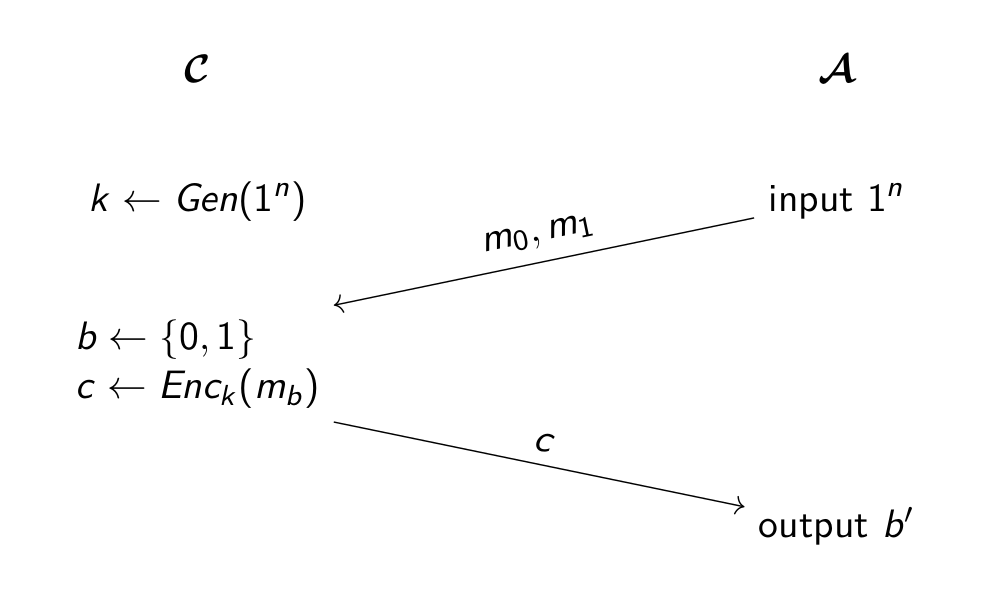
\includegraphics[width=.7\textwidth]{figures/eavesdropping_experiment.png}
\end{figure}
In the eavesdropping experiment, $\mathcal{C}$ first generates a random key $k$.
After that, $\mathcal{A}$ sends them two messages $m_0$ and $m_1$ for encryption with $|m_0| = |m_1|$.
$\mathcal{C}$ then chooses one of the two messages and encrypts it.
If $\mathcal{A}$ can tell which message $\mathcal{C}$ chose, the attack was successful.
If this happens with probability $0.5 + negligible$ the used cipher is secure.

\paragraph{Chosen-plaintext Attack}
\begin{figure}[H]
  \centering
  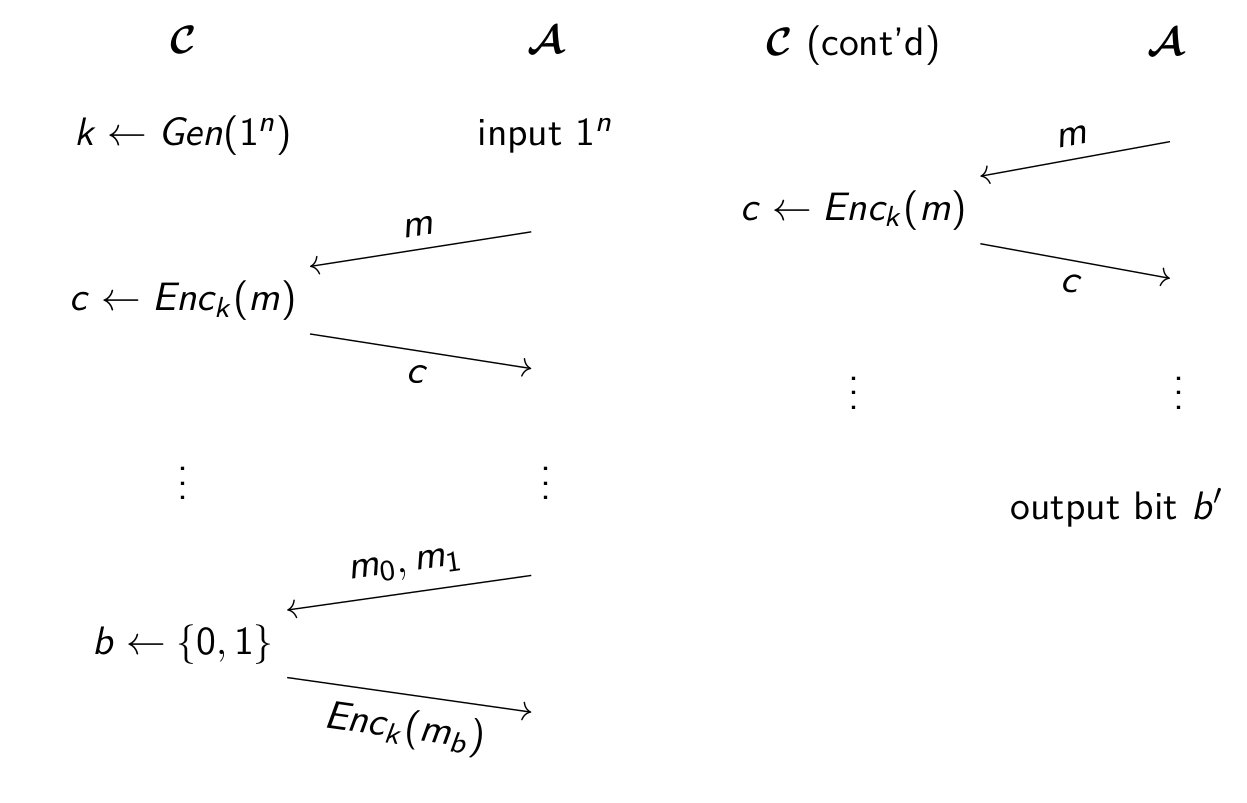
\includegraphics[width=.8\textwidth]{figures/cpa.png}
\end{figure}
In the chosen-plaintext attack the fist step again is that $\mathcal{C}$ generates a random key k.
$\mathcal{A}$ is then allowed to send an arbitrary amount of messages to $\mathcal{C}$ who will encrypt and send them back to $\mathcal{A}$ which means that $\mathcal{C}$ is an ``oracle'' for $\mathcal{A}$.
At some point, $\mathcal{A}$ will send two messages $m_0$ and $m_1$ of equal length of which $\mathcal{C}$ chooses one, encrypts it and sends the result back to $\mathcal{A}$.
$\mathcal{A}$ is then again allowed to use $\mathcal{C}$ as oracle for an arbitray amount of messages and if they are at some point able to tell which message ($m_0$ or $m_1$) $\mathcal{C}$ encrypted, the attack is successful.


\subsubsection{Block and Stream Ciphers}
A block cipher encrypts and decrypts inputs of length $n$ to outputs of length $n$ ($\Rightarrow$ block length $n$).
A steam cipher on the other hand generates a random bitstream with arbitrary length, called keystream, that is xored to the plain text to encrypt and decrypt.\\
The most advisable cipher to use is probably the AES block cipher.
It is well tested and proven to be (mostly) secure and hardware supported what makes it quite fast ($>2GB/s$ with HW support, $200Mbit/s$ without).

\subsubsection{Modes of Encryption}
Modes of encryption are necessary to handle messages of variable length with block ciphers.
The plaintext therefore is split into parts of length equal to the cipher block length.
If the last block is shorter than the block length, we add padding.

\paragraph{Electronic Code Book Mode (ECB)}
\begin{figure}[H]
  \centering
  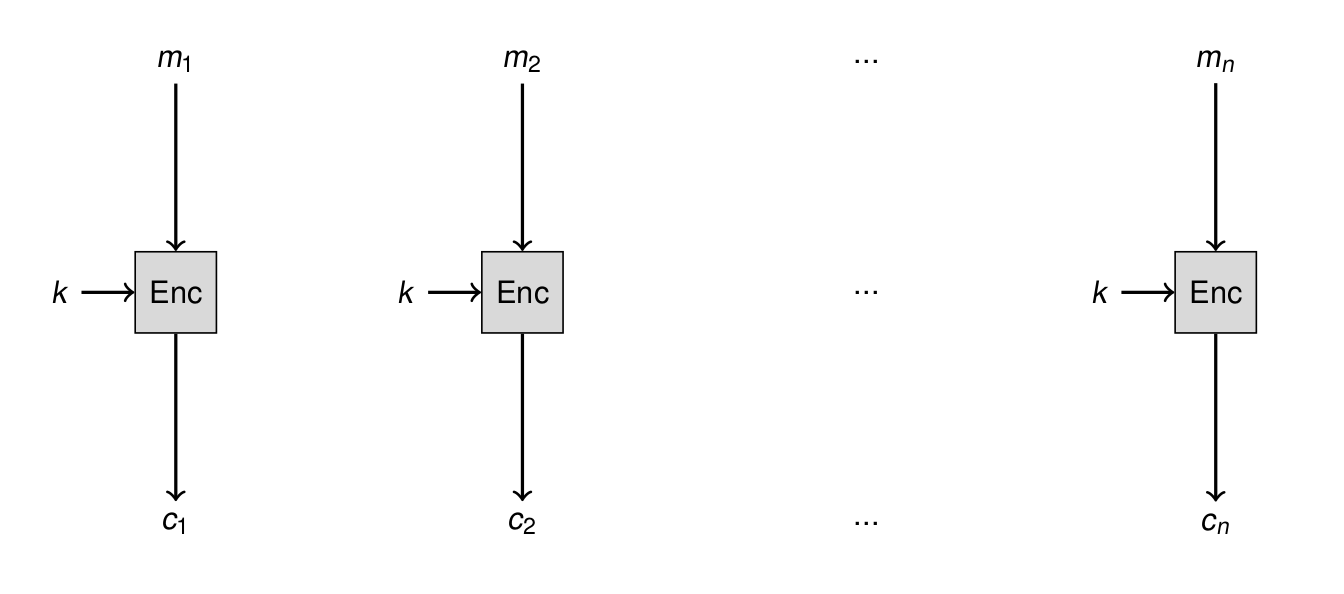
\includegraphics[width=.8\textwidth]{figures/ecb.png}
\end{figure}
In ECB, every plaintext block is encrypted with the unmodified key as input.
The problem thereby is that identical plaintext blocks result in the same ciphertext blocks.
\begin{figure}[H]
  \centering
  
\includegraphics[width=.8\textwidth]{figures/ecb_problem.png}
\end{figure}

\paragraph{Cipher Block Chaining Mode (CBC)}
\begin{figure}[H]
  \centering
  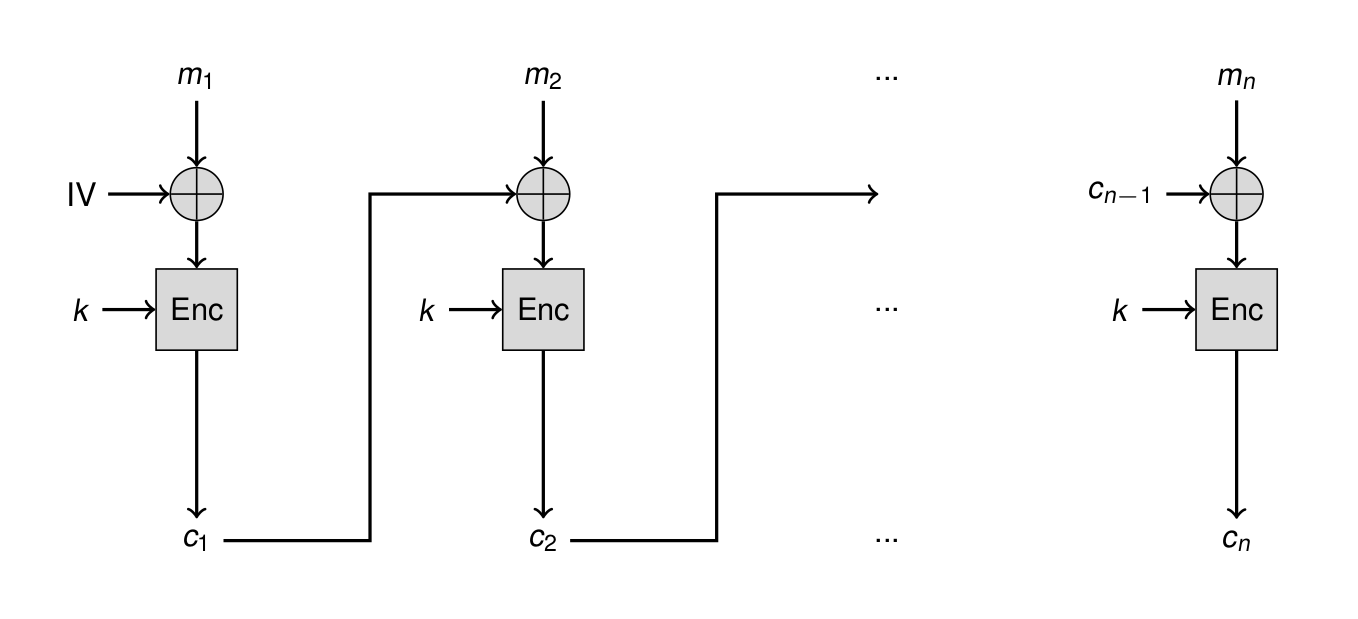
\includegraphics[width=.8\textwidth]{figures/cbc_encrypt.png}
  \caption{CBC Encrypt}\label{fig:cbc_encrypt}
\end{figure}
CBC uses the ciphertext from the previous block xored with the current message block and the unmodified key k as inputs of the encryption function $c_i = Enc_k(c_{i-1} \oplus m_i)$.
For the first message, where no previous cipher block is available, an initialization vector (IV) is used which may be sent in plaintext and is fresh for every massage (or packet if the message is split across multiple packets).\\
Compared to ECB, the advantage is that equal plaintext blocks/messages are not encrypted to the same ciphertext blocks/messages.
\begin{figure}[H]
  \centering
  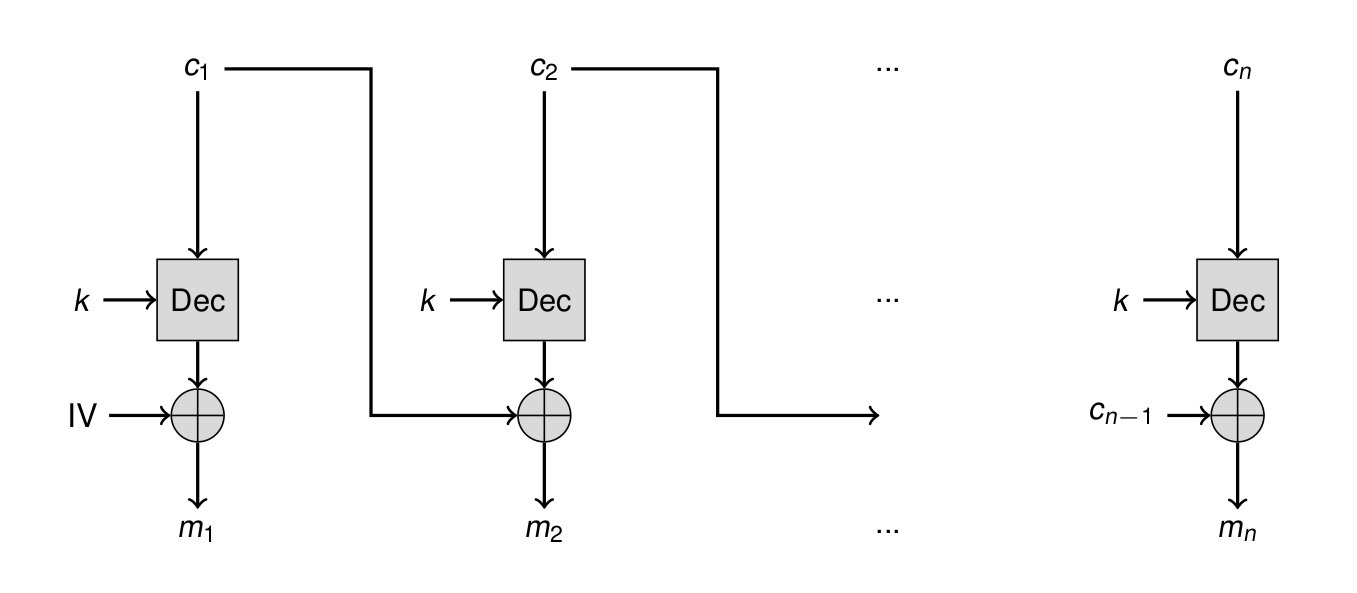
\includegraphics[width=.8\textwidth]{figures/cbc_decrypt.png}
  \caption{CBC Decrypt}
\end{figure}
Decryption is defined by $m_i = c_{i-1} \oplus Dec_k(c_i)$.

\paragraph{Output Feedback Mode (OFB)}
\begin{figure}[H]
  \centering
  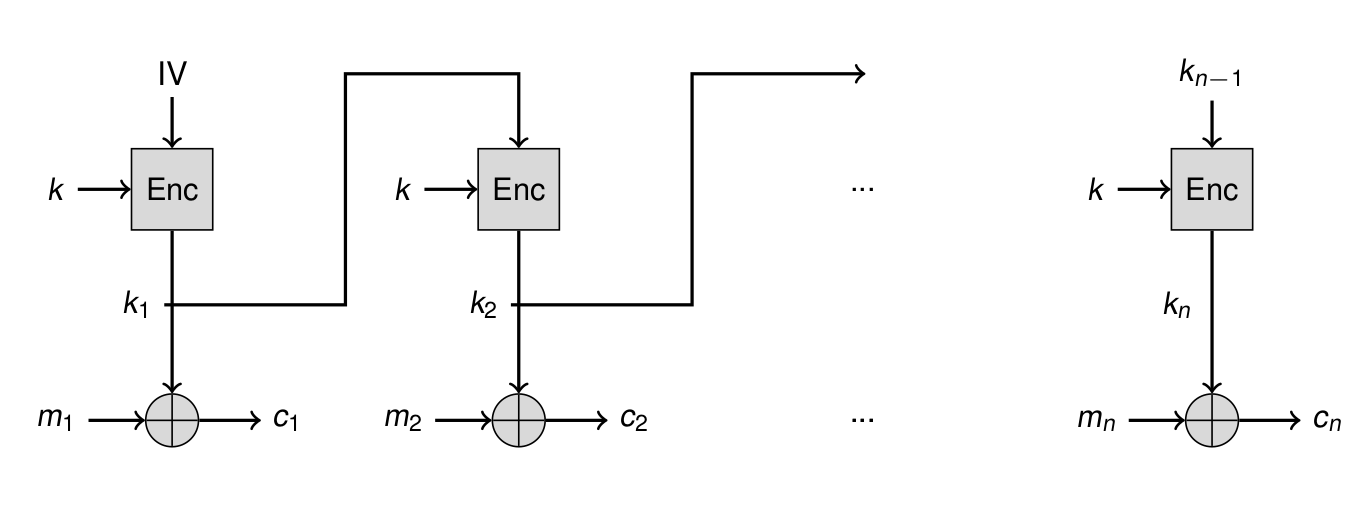
\includegraphics[width=.8\textwidth]{figures/ofb_encrypt.png}
  \caption{OFB Encrypt}
\end{figure}
OFB transforms a block cipher into a stream cipher.
In step $i$, it takes cipher key $k_{i-1}$ form the previous step and encrypts it with the key k.
This cipher key $k_i$ is then xored with the corresponding plaintext block $m_i$ to calculate the ciphertext $c_i$.
In the first step an IV is used as $k_{i-1}$.

\begin{figure}[H]
  \centering
  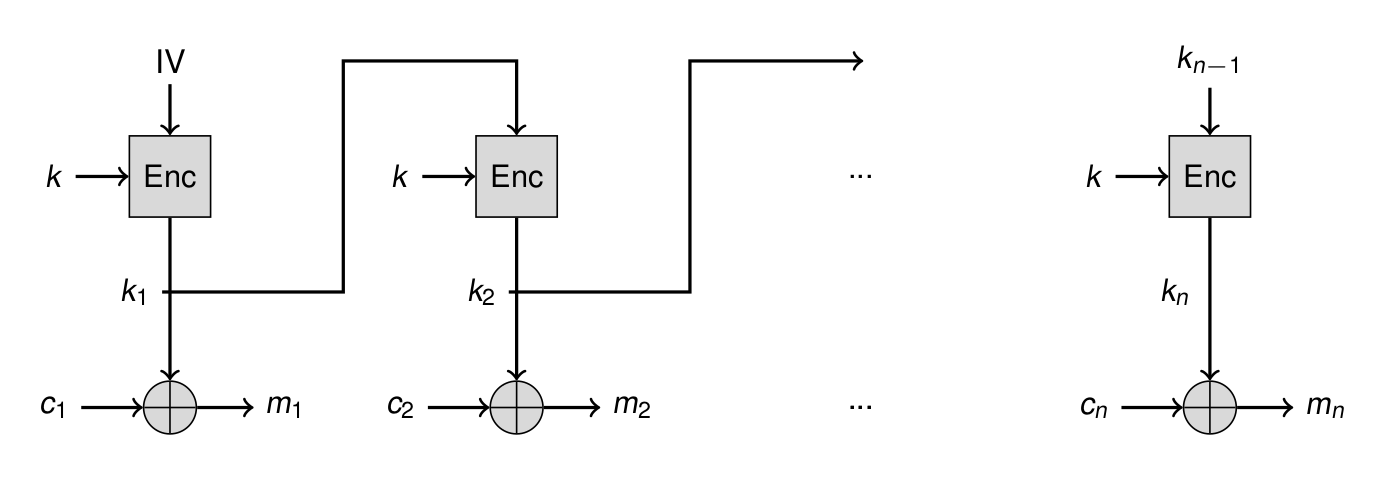
\includegraphics[width=.8\textwidth]{figures/ofb_decrypt}
  \caption{OFB Decrypt}
\end{figure}
Decryption is the same procedure except that the key stream is xored with the cipher text blocks.

\paragraph{Counter Mode (CTR)}
\begin{figure}[H]
  \centering
  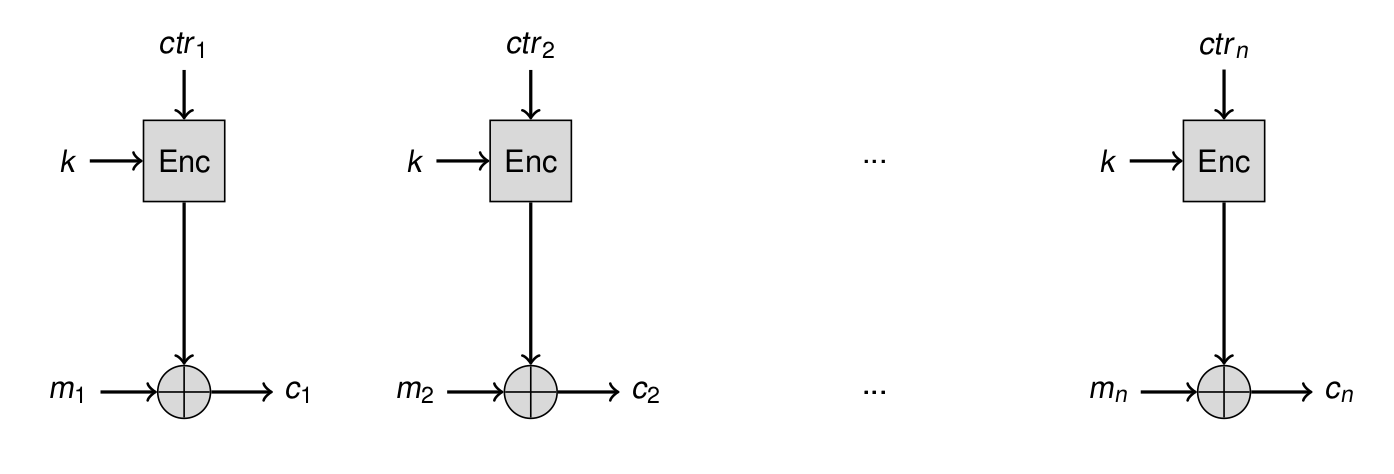
\includegraphics[width=.8\textwidth]{figures/ctr_encrypt}
  \caption{CTR Encrypt}
\end{figure}
In step $i$, CTR encrypts a counter $ctr_i = IV || i$ with key k and xors the result with the plaintext block $m_i$.
Like OFB, CTR also transforms block ciphers into stream ciphers.

\begin{figure}[H]
  \centering
  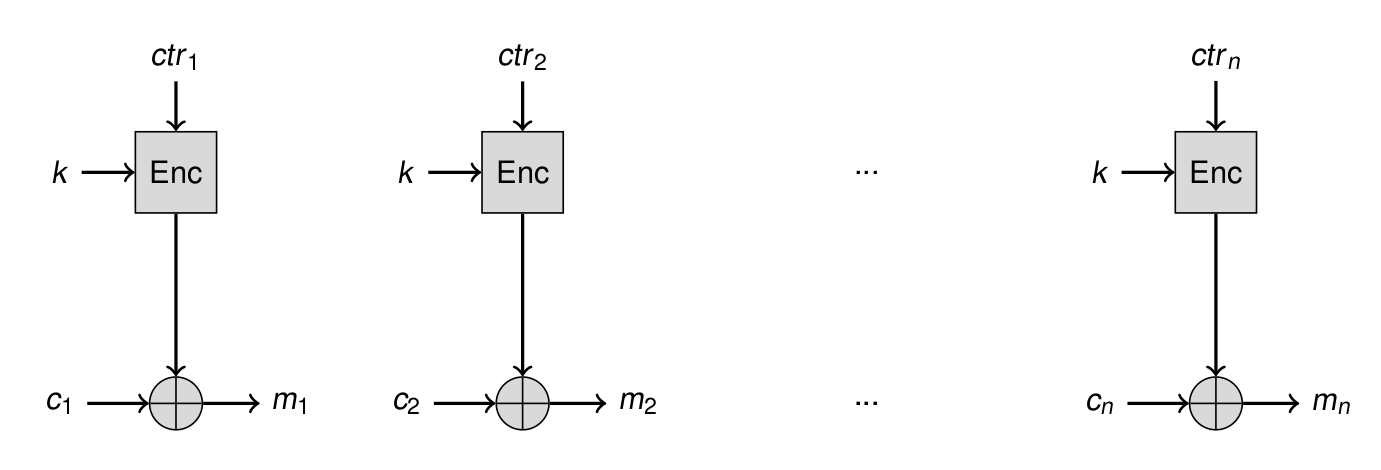
\includegraphics[width=.8\textwidth]{figures/ctr_decrypt.png}
  \caption{CTR Decrypt}
\end{figure}
Decryption is done by $m_i = Enc_k(ctr_i) \oplus c_i$.

\subsubsection{Message Authentication Code (MAC)}
MACs are used in symmetric cryptography to ensure message authenticity but do not provide replay protection.
They are transmitted with the message $\langle m,t \rangle$.
In practice, MACs are either based on hash functions (HMAC), CBC or included in the encryption (authenticated encryption modes).

We define the following terminology:
\begin{itemize}[noitemsep,topsep=0pt]
  \item Key $k \leftarrow Gen(1^n)$
  \item Tag $t \leftarrow Mac_k(m)$
  \item Verification $b := Vrfy_k(m,t)$ where $b=1$ means valid and $b=0$ invalid
\end{itemize}

We define a MAC as secure, if it withstands the adaptive chosen-message attack.

\paragraph{Adaptive Chosen-message Attack}
\begin{figure}[H]
  \centering
  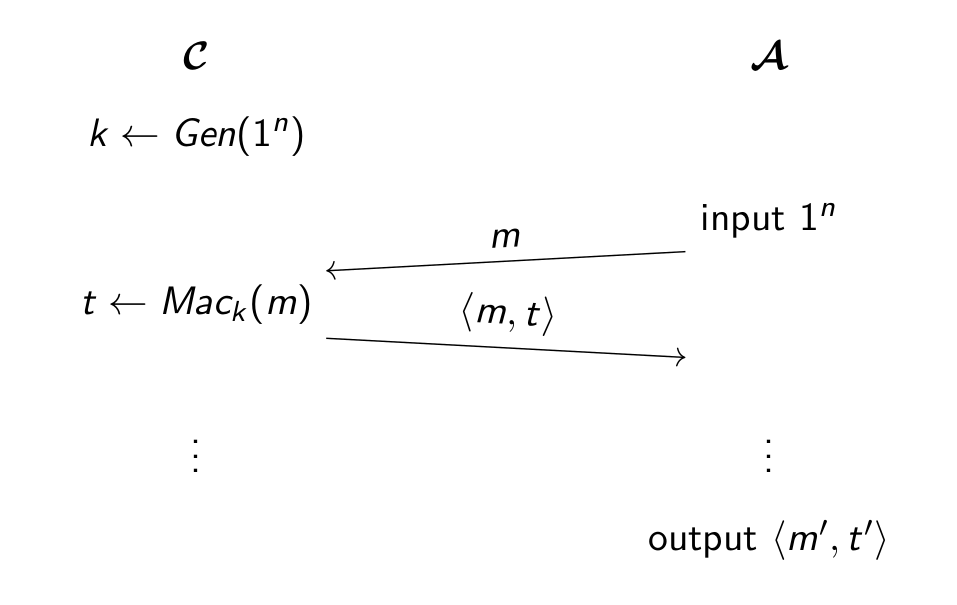
\includegraphics[width=.7\textwidth]{figures/adaptive_chosen-message_attack.png}
\end{figure}
In the adaptive chosen-message attack $\mathcal{C}$ first generates a random key $k$.
$\mathcal{A}$ then sends an arbitrary amount of messages to $\mathcal{C}$ for which they answer with a message consisting of the original message and a tag $t$.
At some point, $\mathcal{A}$ will generate a message-tag pair $\langle m',t' \rangle$ where $m$ was not previously sent to $\mathcal{C}$
The attack is successful, iff $Vrfy_k(m',t') = 1$, so if $\mathcal{A}$ was able to generate a valid MAC tag for a new message.

\paragraph{Hash MAC (HMAC)}
HMAC uses cryptographic hash functions to calculate the MAC\@.
It is calculated with
\begin{equation*}
  t = H(K \oplus opad~|~H(K \oplus ipad | m))
\end{equation*}
To note here is that $K$ is first extended to the block length required for the input of the hash function by appending zeros.
$opad$ and $ipad$ are arbitrary values with the restriction that they have a large Hemming distance to each other.\\
Another note: $H(K~|~m)$, $H(m~|~K)$ or $H(K~|~p~|~m~|~K)$ are not secure.

\paragraph{CBC-MAC}
CBC-MAC encrypts the message to authenticate with another key than used for encryption and uses the last ciphertext block as MAC\@.
CBC is shown in Figure~\ref{fig:cbc_encrypt}.
If the length of a message is not known or no other protection exists, CBC-MAC can be prone to length extension attacks.
CMAC resolves this.

\paragraph{CMAC}
CMAC is an improved version of CBC-MAC which has to keys, calculated from the shared key, where one is used for xoring with complete bocks before encryption and the other one for incomplete blocks.
XCBC-MAC is another improvement of this where the two keys are input to the algorithm and not derived from k.

\subsubsection{Combining Confidentiality and Authentication}
Generally the best approach to combine confidentiality and authentication is to first encrypt and then authenticate, i.e.\ $c \leftarrow Enc_{k_1}(m)$, $t \leftarrow Mac_{k_2}(c)$ and transmit $\langle c,t \rangle$.

\subsection{Asymmetric Cryptography}
In asymmetric cryptography, the two communication partners no longer have one shared key, but each participant has a key pair.
A private/secure key (sk) that is only known to one person and is used for decryption and message signing and a public key (pk) that can be published and is used for encryption and message verification.
Asymmetric cryptography is based on mathematical problems which are believed to be hard (e.g.\ integer factorization).
It only needs an authenticated channel to exchange keys of which less amounts are required than in the symmetric setting.
It is orders of magnitudes slower though.

\subsubsection{Public-key Encryption Scheme}
\begin{enumerate}
  \item $(pk,sk) \leftarrow Gen(1^n)$
  \item Encryption with public key: $c \leftarrow Enc_{pk}(m)$
  \item Decryption with private key: $m := Dec_{sk}(c)$
\end{enumerate}

\paragraph{RSA}
Key generation in RSA is done with the following procedure:
\begin{enumerate}
  \item $(N,p,q) \leftarrow GenModulus(1^n)$
  \item $\phi(N) := (p-1)(q-1)$
  \item find $e$: $\gcd(e,\phi(N)) = 1$
  \item $d := [e^{-1} \mod \phi(N)]$
  \item $pk = \langle N,e \rangle$
  \item $sk = \langle N,d \rangle$
\end{enumerate}

Encryption then is defined as $RSA_{pk}(y) := [y^e \mod N]$ and decryption as $RSA_{sk}(y) = [z^d \mod N]$.

\paragraph{Chosen-ciphertext Attack (CCA)}
An asymmetric encryption scheme is considered secure if it withstands CCA\@.
\begin{figure}[H]
  \centering
  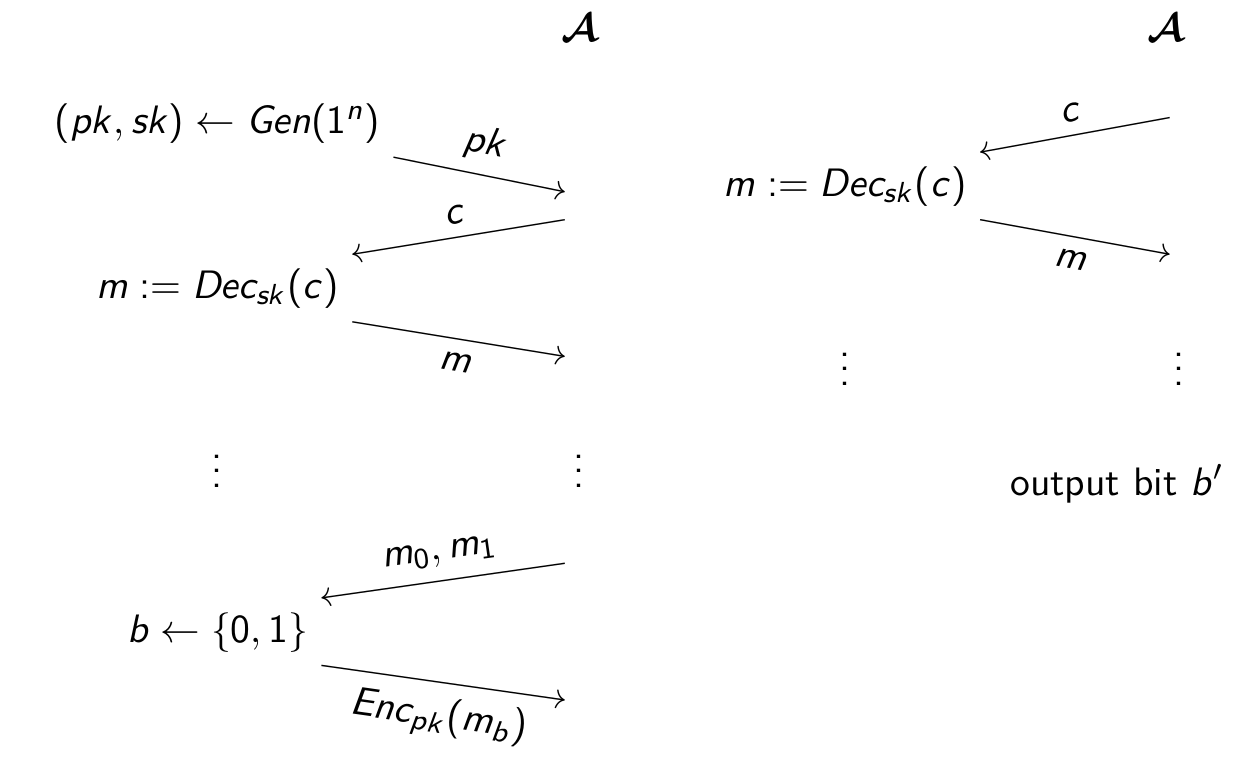
\includegraphics[width=.8\textwidth]{figures/cca.png}
\end{figure}
CCA is quite similar to CPA except $\mathcal{A}$ sends ciphertext messages to $\mathcal{C}$ for probing instead of plaintext ones.
A restriction not depicted in the illustration above is that $\mathcal{A}$ may not request a decryption for $Enc_{pk}(m_b)$ itself.
\newpage

\paragraph{Optimal Asymmetric Encryption Padding (OAEP)}
OAEP is a padding scheme for asymmetric encryption depicted below.
\begin{figure}[H]
  \centering
  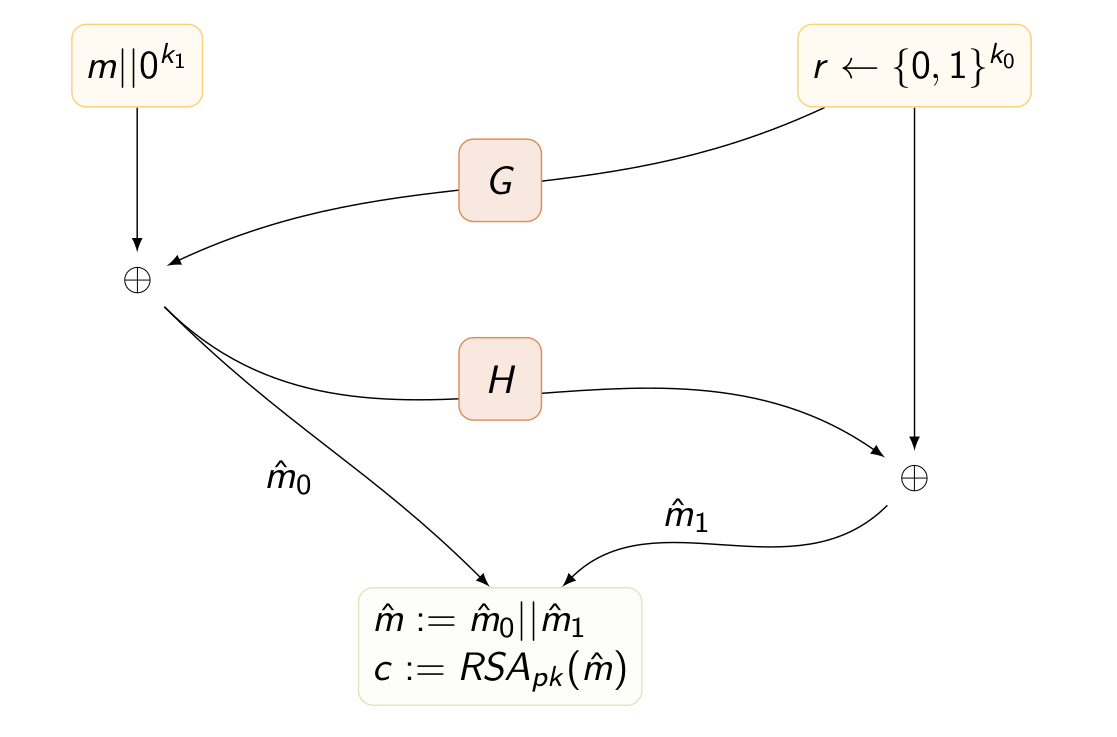
\includegraphics[width=.7\textwidth]{figures/oaep.png}
\end{figure}

RSA used in conjunction with OAEP is secure under CCA\@.

\subsubsection{Signature Scheme}
\begin{enumerate}
  \item $(pk,sk) \leftarrow Gen(1^n)$
  \item Signature generation with private key: $\sigma \leftarrow Sign_{sk}(m)$
  \item Signature verification with public key: $b := Vrfy_{pk}(m,\sigma)$ where $b = 1$ means valid and $b = 0$ invalid
\end{enumerate}
Signatures are often slower than their MAC relatives and provide non-repudiation.
A signature scheme is considered secure if it withstands the adaptive chosen-message attack.
\newpage

\paragraph{RSASSA-PSS}
RSASSA-PSS is a signature scheme that uses RSA\@.
\begin{figure}[H]
  \centering
  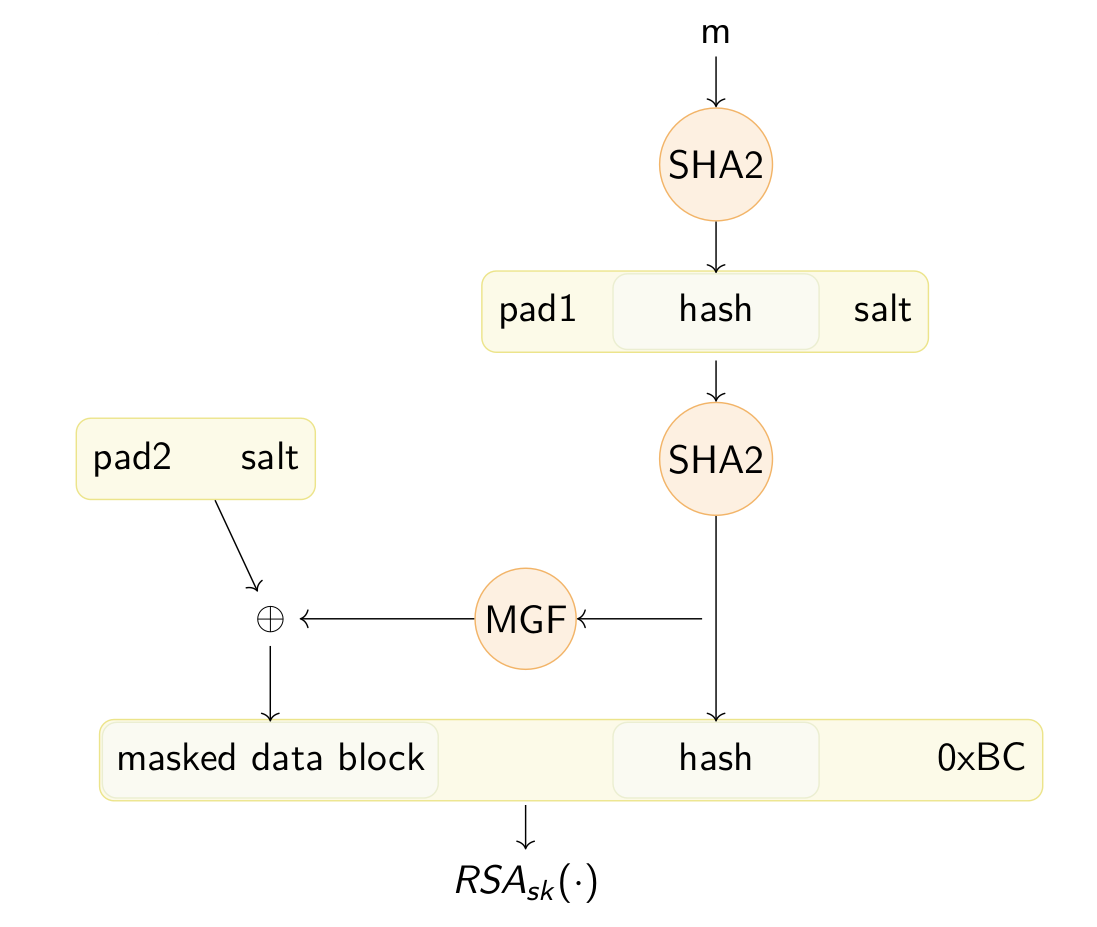
\includegraphics[width=.8\textwidth]{figures/rsassa-pss.png}
\end{figure}
RSASSA-PSS is secure under adaptive chosen-message attack and breaking it would mean that RSA is broken.

\subsection{Hybrid Approach}
Since public key cryptography is slower than secret key cryptography, a hybrid approach is often advisable.
Public-key cryptography is used to protect a shared key (session key) that is used for any further communication via secret-key cryptography.
They private key for the key exchange is called long-term key.\\

\textbf{Perfect forward secrecy} is often an important property of this approach.
It states that if an attacker gains access to the long-term key or the session key, they should not be able to decrypt messages of past sessions.\\

A common strategy is to use a signed Diffie-Hellman key exchange and a secret-key authenticated encryption scheme for communication.
To guarantee perfect forward secrecy, DH keys have to be calculated for every connection and old keys have to be wiped.
\newpage

\subsubsection{Diffie-Hellman Key Exchange (DH)}
\begin{figure}[H]
  \centering
  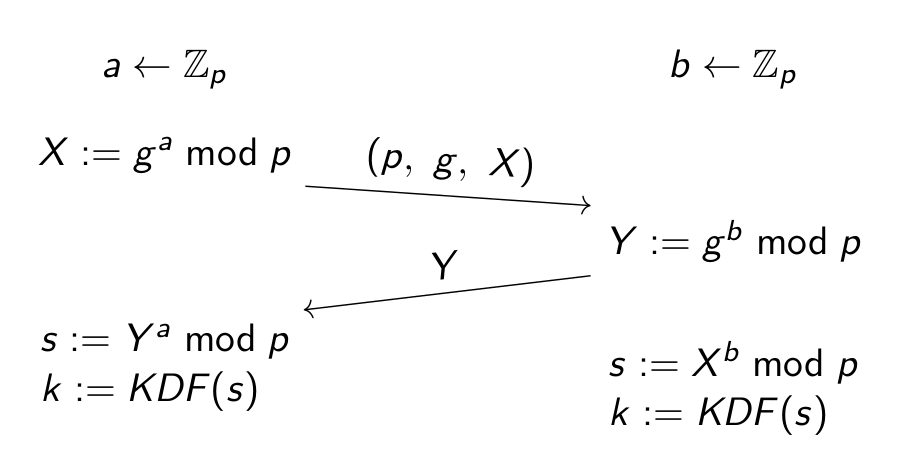
\includegraphics[width=.7\textwidth]{figures/diffie-hellmann.png}
\end{figure}
In the first step of the DH key exchange, communication partner A selects a prime $p$, a generator $g$ which is a primitive root for the cyclic group of $\mathds{Z}_p$ and a random number $a \in \mathds{Z}_p$.
A then calculates $X = g^a \mod p$ and sends it with $p$ and $g$ to B.
B also chooses a random number $b \in \mathds{Z}_p$ and calculates $Y = g^b \mod p$ which they send back to A.
Both can then calculate the key $k$ by $k = Y^a = g^{ba} = g^{ab} = X^b~\mod p$.
